%\documentclass{cmspaper}
%\begin{document}
\section{Jet Studies} \label{sec:jet}
%from : /twiki.cern.ch/twiki/bin/view/CMS/WorkBookJetAnalysis

\subsection{Jet Algorithm and Cleaning}
%monicava.web.cern.ch/monicava/Talks/JetTutorial130.pdf
%http://64.233.169.104/search?q=cache:ON_R5d7inNQJ:arxiv.org/pdf/0705.2696+iterative+cone+algorithm&hl=en&ct=clnk&cd=1&gl=us&client=firefox-a

The jet reconstruction algorithm used in this analysis is an iterative cone algorithm using a radius of $\Delta R=0.5$ \cite{JetAlg}.  
The algorithm starts with seeds in calorimeter towers (combining ECAL and HCAL) with energies greater than 
1 GeV. It then considers the weighted average of all energy in a cone of radius 0.5 around this seed to form a proto-jet.  
A cone of $\Delta R = 0.5$ is then constructed around the momentum vector of each new proto-jet,  
and the process is continued iteratively until a stable jet four-vector is obtained.

%########Both mass at p must stabilize, or just the three-vector???????????

This algorithm also provides high energy "electrons" to be included in the jet collection. 
To remove such electrons ("cleaning") the collection of electrons that pass electron ID and Isolation 
selection criteria is created, as described in Section~\ref{sec:electrons}. The three-vectors of the 
electrons in this new collection is then compared to the three-vectors of the jets. 
A jet is removed if it is within a $\Delta R$ of 0.5 from one of the electrons. 
Figure~\ref{fig:JetCleaning} shows the distribution of the number of reconstructed jets 
per event with $P_{T}>50$ GeV and $|\eta|<3$ for a sample of LQ with mass of 400 GeV, before and after cleaning procedure; 
the whole distribution is shifted on the left by two units after the cleaning, since the two real electrons 
coming from LQ decays are correctly removed from the jet list. 

%   1.  convert ADC counts to energy in one calorimeter cell
%          * HcalSimpleReconstructor does this calculation for HCAL
%          * ECAL does it in two steps
%                o first produces uncalibrated hits: EcalWeightUncalibratedRecHitProducer
%                o then calibrates hits: EcalAnalFitUncalibratedRecHitProducer 
%   2. combine ECAL and HCAL cells into projective towers corresponding to HCAL granularity
%          * CaloTowersCreator does this operation 
%   3. convert CaloTowers into standard objects CaloTowerCandidateCreator (see more details in the next section)
%   4. run clustering algorithm to produce Jets
%          * Several basic algorithms and corresponding producers are currently implemented for CMS
%                o Midpoint Cone algorithm: midpointJetProducer <-- used in this tutorial
%                o Iterative Cone algorithm: iterativeConeJetProducer
%                o KT algorithm: ktJetProducer
%                o Seedless Infrared Safe cone algorithm: sisConeProducer 

\subsection{Jet Energy Corrections}

The corrections for the Jet Energy Scale (JES) are divided into various levels in the CMS Software \cite{JES}.  
In this analysis the jet energy is corrected with the level 2, 3, and 5 corrections.

The Level 2 jet energy corrections comprise the 
``relative jet corrections'' that provide uniform jet energy response in $\eta$.  
The Level 3 corrections are the ``absolute jet corrections'', that aim to correct  the jet energies 
%in the region of $\eta < 1.3$ 
back to the particle level energy, to assure agreement in energy with the generated MC samples. 
Figure~\ref{fig:CorrRatios}(a) shows the ratio of distributions in jet energies after and before implementing  
the combination of absolute and relative corrections.  
The relative and absolute corrections are the standard CMS Software corrections recommended for all jet analyzes,
and on average change the energies by 20\%.

In addition, Level 5 corrections are applied to take account of the flavor of the originating parton.
Figure~\ref{fig:CorrRatios}(b) shows the mean additional correction factor (beyond the relative and absolute corrections) 
for the jets based on the corrections of light quarks, which change the overall energy of jets by only a few percent.

The relative and absolute corrections are based on samples enriched in gluon jets (as in QCD multi jet events) but jets from 
first-generation LQ decays arise from light quarks.  Since the gluon-jets have
a softer fragmentation function, the level 2 and 3 corrections tend to overcompensate the loss of energy when applied to jets originated 
from quarks. This is the reason why the level 5 corrections for light quarks decrease the average energy of the jet, 
as shown in Figure~\ref{fig:CorrRatios}-right. 

The optional Level-4 corrections aim to correct the fraction of energy deposited in the EM section of the calorimeter, 
a quantity not used in this analysis, and therefore not applied.
%Level 7 corrections correct the energy of a jet back to the energy of its parton.
%This is based on specific production processes, such as light quark jets from dijet production or charm quarks from ttbar decays.  
%There is no general correction function of this kind available for a LQ analysis.
%%%%%%%%%%%
%FIXME% Add plot of Mej distribution for matched electrons and jets from 400 GeV LQ decay, before and after JES corrections.
%%%%%%%%%%%

\begin{figure}
  \begin{center}
  \begin{tabular}{cc}
    \resizebox{10cm}{!}{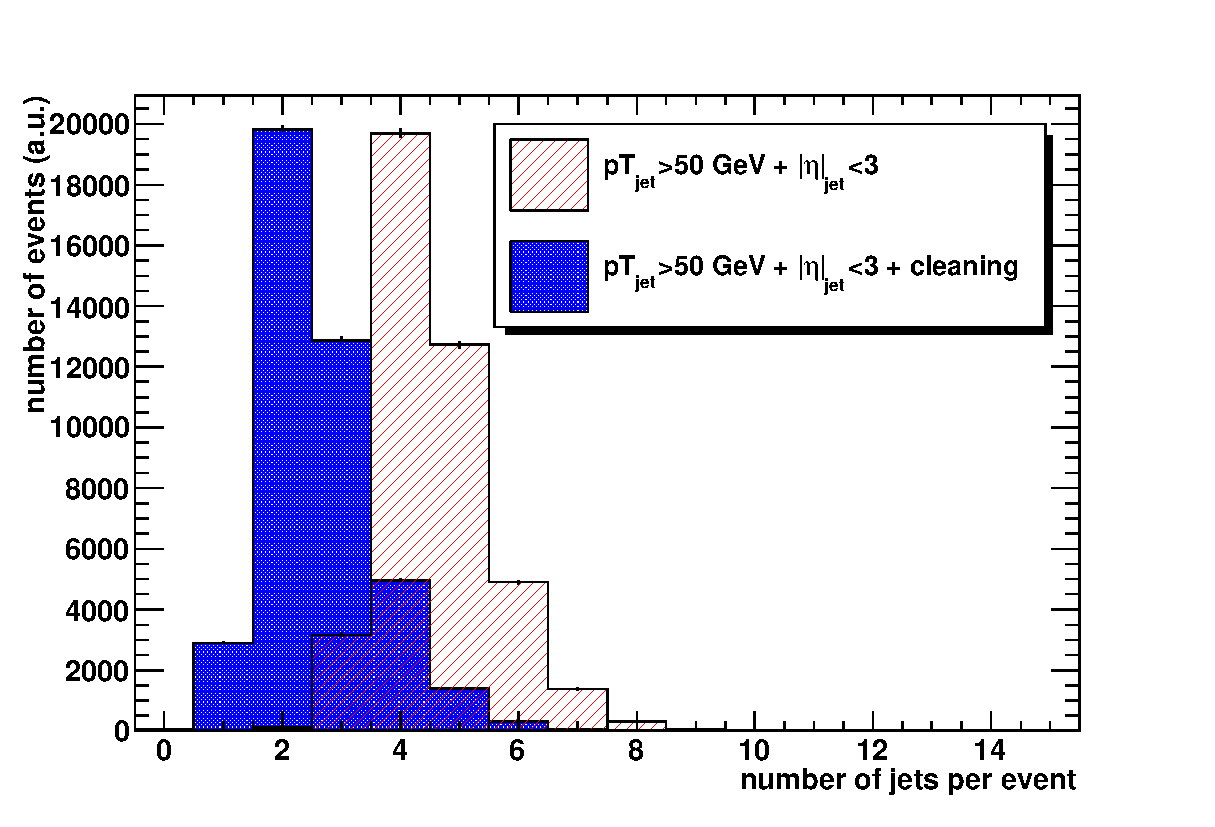
\includegraphics{plots/JetPlots/Njets.eps}} \\
  \end{tabular}
  \caption{\small \sl The distribution of the number of reconstructed jets 
    per event with $P_{T}>50$ GeV and $|\eta|<3$ for a sample of LQ with mass of 400 GeV, before and after cleaning procedure; 
    the whole distribution is shifted on the left by two units after the cleaning, since the two real electrons 
    coming from LQ decays are correctly removed from the jet list.}
    \label{fig:JetCleaning}
  \end{center}
\end{figure}

%FIXME % put new plots of JES corrections (Ellie)

\begin{figure}
  \begin{center}
  \begin{tabular}{cc}
    a.
  \resizebox{8cm}{!}{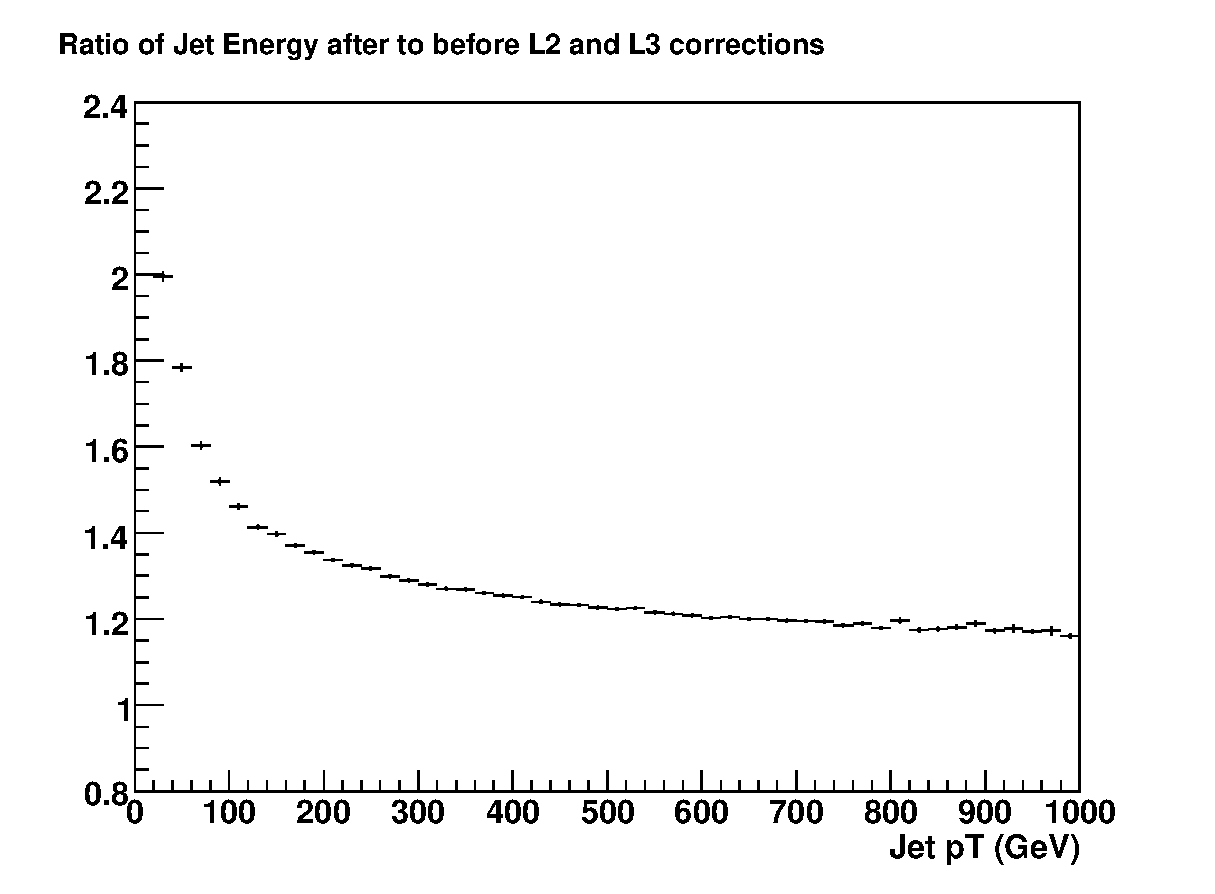
\includegraphics{plots/L23Raw_OLDNOTE.eps}}                  &
   b.
  \resizebox{8cm}{!}{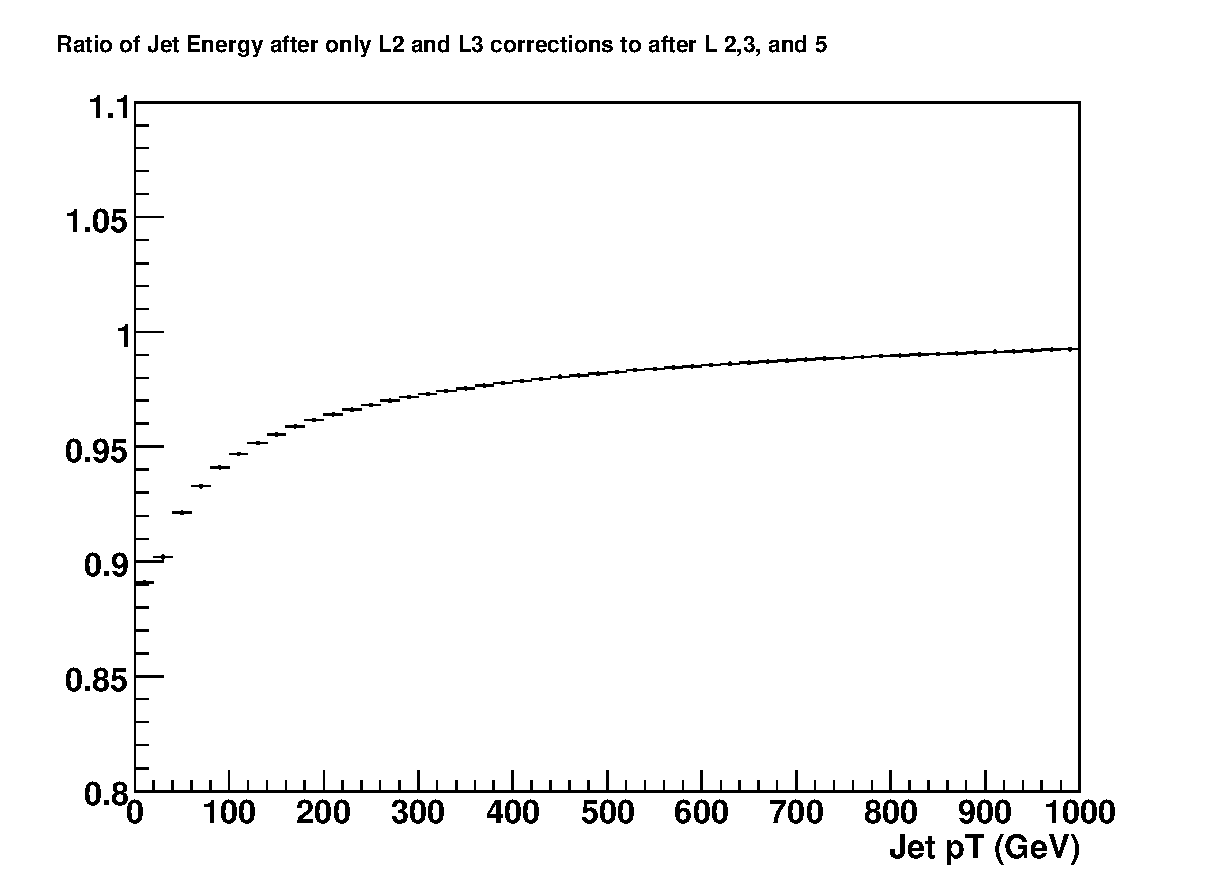
\includegraphics{plots/L5L23_OLDNOTE.eps}} \\
  \end{tabular}
  \caption{\small \sl a - Mean ratio of jet energy after the level 2 and 3 corrections to that with no correction as a function of $P_T$. b 
    - Ratio of jet energy after the level 2,3, and 5 corrections to that with only level 2 and 3 corrections as a function of $P_T$.  
    Plots show the average correction for all jets in each $P_T$ bin.  These jets are taken from a LQ sample with a mass of 400 GeV.}
    \label{fig:CorrRatios}
  \end{center}
\end{figure}

%\subsection{Efficiencies}

%The reconstruction efficiency of the jets from the leptoquark decays is quite high in the fiducial volume of the barrel and endcap.  Fortunately, the majority of the jets from the leptoquark decay are central 
%(see figure~\ref{fig:jetVariables}).  The barrel region for CMS ends at $\eta = 1.3$, so any objects hitting the detector in this region will have a much greater likelihood of being properly reconstructed.  
%Figure\ref{fig:jetEffFV} shows that for any jets within the barrel region with a pT greater than approximately 50 GeV the reconstruction efficiency is better than 90\%.  The efficiency in the endcap region is 
%slightly lower, but still quite good.  The jet efficiency is shown to be high enough that no optimization of the cuts on jet variables has yet been done.  
 
%  \begin{figure}
%    \begin{center}
%    \begin{tabular}{cc}
%      \resizebox{0.3\linewidth}{!}{\includegraphics{plots/JetEffEta.eps}} &
%      \resizebox{0.3\linewidth}{!}{\includegraphics{plots/JetEffPt.eps}}
%     \end{tabular}
%      \caption{\small \sl Efficiency of Jet Reconstruction of jets from a LQ of mass 650 GeV with respect to $\eta$ and $P_T$}
%      \label{fig:jetEffFV}
%    \end{center}
%  \end{figure}
 

%  \begin{table}[htb]
%    \caption{\small \sl Electron Acceptance-Efficiency (FastSim)}
%    \label{tab:JetEffAcc}
%    \begin{center}
%      \begin{tabular}{|l|c|c|c|} \hline
%	    LQ mass (GeV) & $A_{Fiducial Region}$ & $\epsilon_{Fiducial Region}$ & $A\times\epsilon_{Fiducial Region}$\\ \hline
%	    250 & XX\% & XX\% & XX\% \\ \hline
%	    400 & XX\% & XX\% & XX\% \\ \hline
%	    600 & XX\% & XX\% & XX\% \\ \hline
%	    1000 & XX\% & XX\% & XX\% \\ \hline
%      \end{tabular}
%    \end{center}
%  \end{table}
%


%\begin{figure}
%  \begin{center}
%    \begin{tabular}{cc}
%      \resizebox{7cm}{!}{
\includegraphics{plots/UMD.eps}} &
%      \resizebox{7cm}{!}{
\includegraphics{plots/UMD.eps}} \\
%      \resizebox{7cm}{!}{
\includegraphics{plots/UMD.eps}} &
%      \resizebox{7cm}{!}{
\includegraphics{plots/UMD.eps}} \\
%    \end{tabular}
%    \caption{\small \sl Distributions of jet reconstructed quantities in FastSim and Full Sim samples with $M_{LQ}=650$ GeV.  
%      Jets are matched to a quark from a leptoquark by a $\Delta R<0.5$. Only jets with $P_{T}>50$ GeV are considered.
%      From the top left to the bottom right: number of jets per event, number of jets coming from LQ decays per event, 
%    $\eta$, and $P_{T}$.}
%    \label{fig:jetVariables}
%  \end{center}
%\end{figure}

%disambiguation, corrections

%pT, eta dist

%efficiencies (pT, eta)

%fast vs full

%\end{document}
